\documentclass[border=5pt]{standalone}
\usepackage{tikz}
\usepackage{amsmath}
\usetikzlibrary{calc,intersections}
\usepackage{pgfplots}
\pgfplotsset{compat=1.16}
\usepgfplotslibrary{polar}
\begin{document}
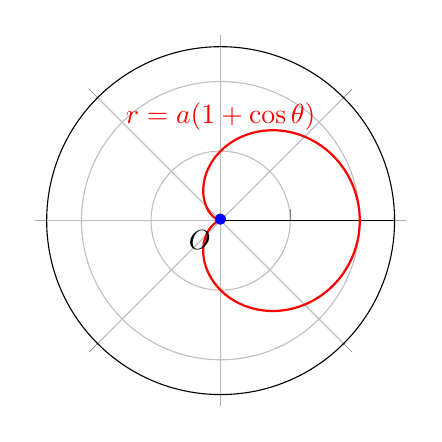
\begin{tikzpicture}
\begin{polaraxis}[
    width=6cm,
    height=6cm,
    grid=both,
    xmin=0, xmax=360,
    ymin=0, ymax=2.5,
    xtick={0,45,...,315},
    ytick={1,2},
    xticklabels={},
    yticklabels={},
]
    % Cardioid r = a(1 + cos θ)
    \addplot[red, thick, domain=0:360, samples=200] {1+cos(x)};

    % Origin
    \node[blue] at (axis cs:0,0) {$\bullet$};
    \node[below left] at (axis cs:0,0) {$O$};

    % Cusp
    \node[blue] at (axis cs:180,0) {$\bullet$};

    % Labels
    \node[red] at (axis cs:90,1.5) {$r = a(1 + \cos\theta)$};
\end{polaraxis}
\end{tikzpicture}
\hspace{0.5cm}
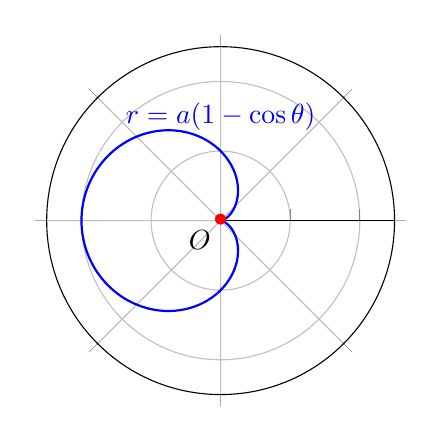
\begin{tikzpicture}
\begin{polaraxis}[
    width=6cm,
    height=6cm,
    grid=both,
    xmin=0, xmax=360,
    ymin=0, ymax=2.5,
    xtick={0,45,...,315},
    ytick={1,2},
    xticklabels={},
    yticklabels={},
]
    % Cardioid r = a(1 - cos θ)
    \addplot[blue, thick, domain=0:360, samples=200] {1-cos(x)};

    % Origin
    \node[red] at (axis cs:0,0) {$\bullet$};
    \node[below left] at (axis cs:0,0) {$O$};

    % Cusp
    \node[red] at (axis cs:0,0) {$\bullet$};

    % Labels
    \node[blue] at (axis cs:90,1.5) {$r = a(1 - \cos\theta)$};
\end{polaraxis}
\end{tikzpicture}
\end{document}
